\section{Conceitos Fundamentais}

\begin{frame}
	\begin{block}{Conceitos Fundamentais}
		 \begin{enumerate}
		  \item Sistemas Gerenciadores de Workflows Científicos.
		  \item Sistemas de recomendação.
		  \item Recomendação em \emph{workflows} científicos.
		  \item Ontologias.
		  \item Recomendação baseada em bases de dados de \emph{workflows} científicos.
		  \item Métricas de validação.
		  \item Recomendação a partir de banco de workflows.
		  \item Classificadores e regressores.
		 \end{enumerate}
	\end{block}
\end{frame}


\begin{frame}
	\begin{figure}[!htb]
		\centering	  				
		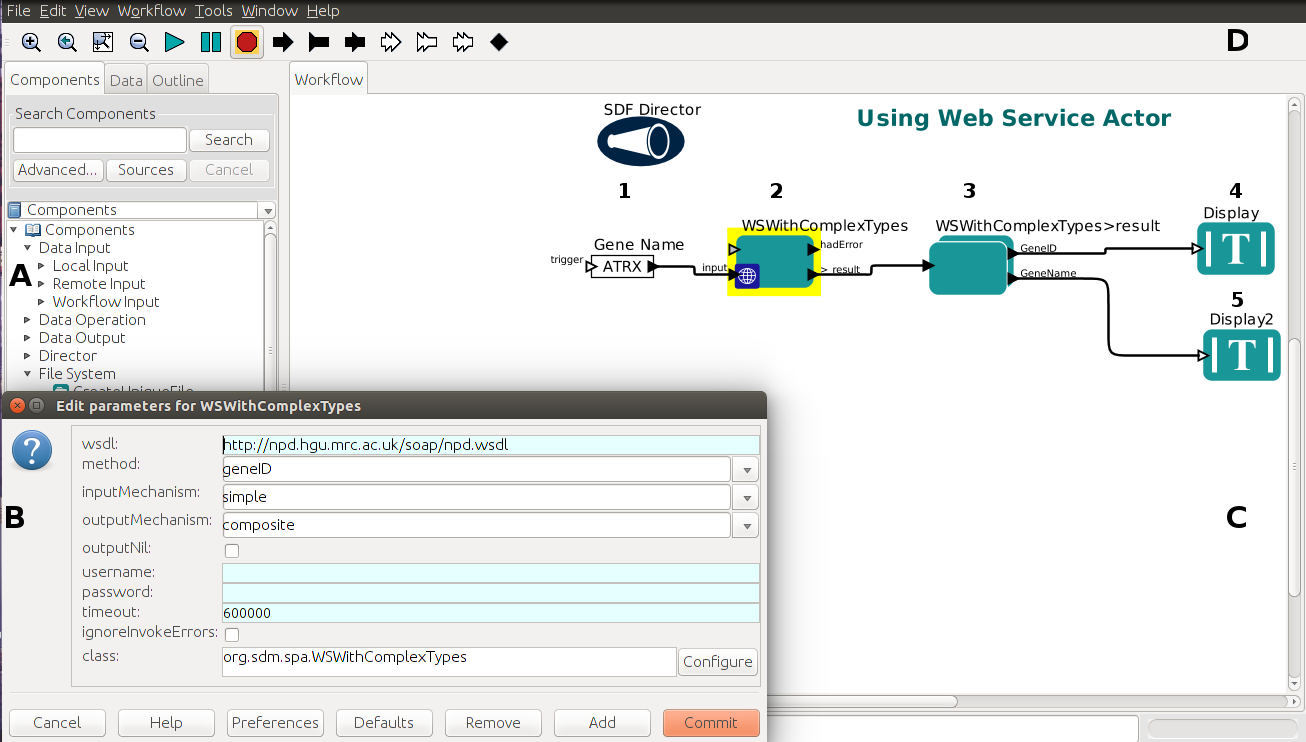
\includegraphics[height=7cm]{./secoes/ConceitosFundamentais/webService.png}
		\caption{Exemplo de sistema gerenciador de \emph{workflow} científico.}
		\label{fig_sistema_gerenciador_workflow_cientifico}
 	\end{figure}
\end{frame}


\begin{frame}		
	\begin{block}{}
		Sistemas de recomendação têm por objetivo \textbf{recomendar itens úteis} para usuários:
		\begin{eqnarray}
		\forall c \in C,  \quad s_{c}^{'} =  \operatorname*{arg\,max}_{s \in S} u(c,s) \label{formalizar_recomendacao}
		\end{eqnarray}
		
		A função utilidade \(u\) não está definida para todo o espaço \(C \times S\), isso força os sistemas de recomendação a extrapolar o espaço conhecido.
	\end{block}
\end{frame}


\begin{frame}
	\begin{block}{}
		Algumas estratégias utilizadas em sistemas de recomendações:
		
		\begin{enumerate}
			\item \emph{Content-based}.
			\item \emph{Collaborative Filter (usuários parecidos)}.
			\item \emph{Hibrid Approach}.
			\item \emph{Community Based (usuários amigos)}.
			\item \emph{Demographic}.
			\item \emph{Knowledge-based}.
		\end{enumerate}
	\end{block}
\end{frame}


\begin{frame}		
	\begin{block}{}
		\textbf{Recomendar atividades em workflows científicos} exige, além da extrapolação citada, considerar as restrições:
		\begin{enumerate}
			\item Dependência entre entrada e saída de atividades.
			\item Dependência semântica.
			\item A ordem das atividades (citar exemplo de sistema de recomendação de música).
		\end{enumerate}
	\end{block}
\end{frame}


\begin{frame}
	\begin{block}{}
		\textbf{Ontologia} é um modelo para representação de conhecimento, a qual, pode ser utilizadas para anotar semanticamente atividades.
		
		\begin{figure}
			\begin{minipage}[b]{0.7\textwidth}
				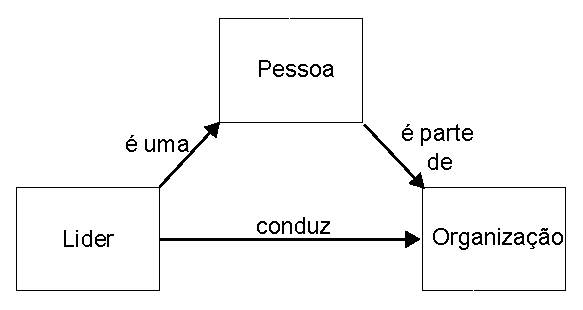
\includegraphics[width=\textwidth]{./secoes/ConceitosFundamentais/Ontologia.eps}
				\caption{Exemplo de Ontologia}
			\end{minipage}
		\end{figure}
	\end{block}
\end{frame}

\begin{frame}
	\begin{block}{}
		Os experimentos serão validados por \emph{10-fold cross validation}, em cada rodada serão calculadas as métricas:
		\begin{enumerate}
			\item \emph{Sucess at rank k} (\(S@k\)).
			\item \emph{Mean Reciprocal Rank} (MRR).		
		\end{enumerate}
		
		\begin{figure}
			\begin{minipage}[b]{0.9\textwidth}
				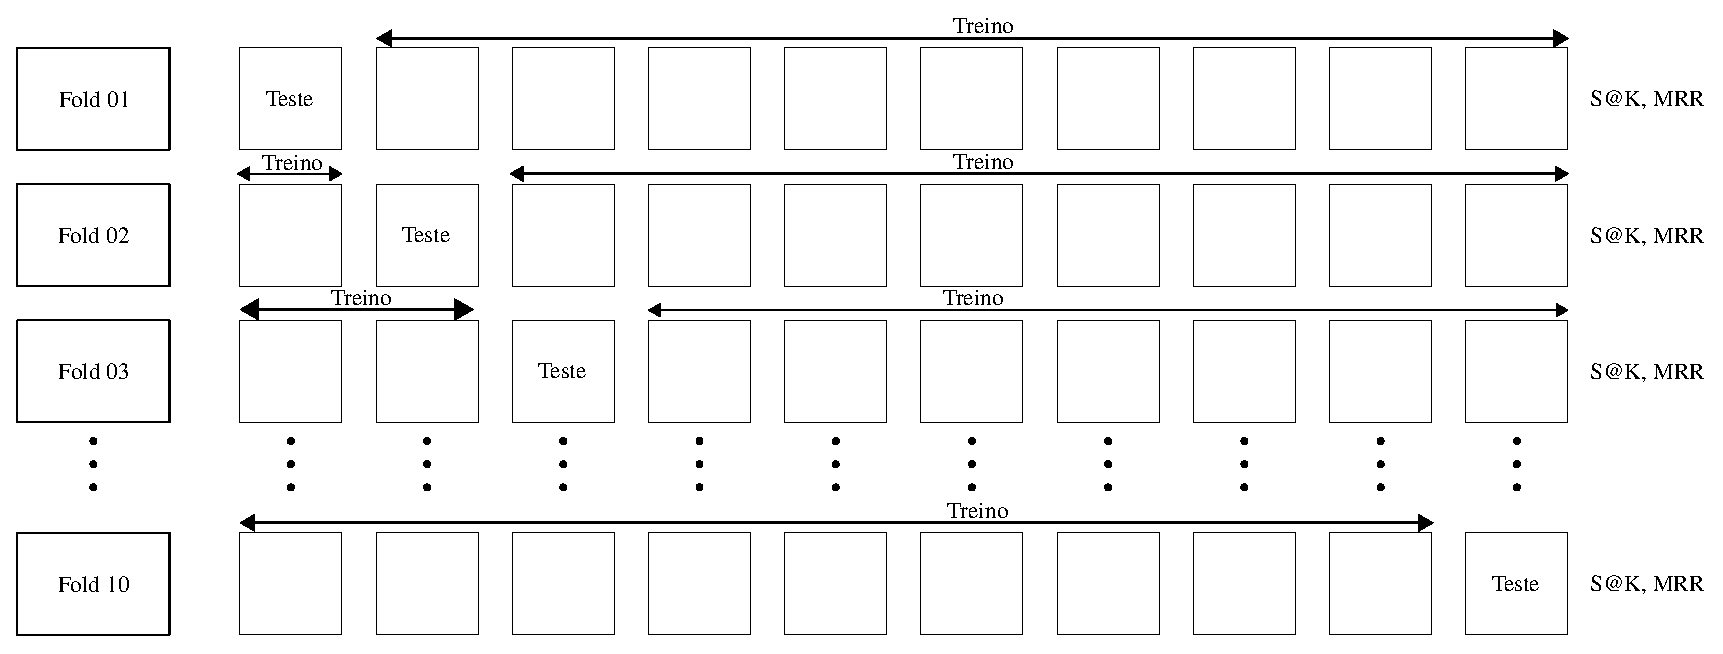
\includegraphics[width=\textwidth]{./secoes/ConceitosFundamentais/10FOLDCROSS.eps}
				\caption{Exemplo de \emph{10-fold cross validation}}
			\end{minipage}
		\end{figure}
		
	\end{block}
\end{frame}

\begin{frame}
	\begin{block}{}
		\textbf{Recomendação a partir de banco de workflows}
		\begin{enumerate}
			\item Frequência;
			\item \emph{itemsets}.	
		\end{enumerate}
	\end{block}
\end{frame}


\begin{frame}
	\begin{block}{}
		\textbf{Recomendação a partir de classificadores}
		\begin{enumerate}
			\item CART;
			\item KNN;
			\item Naive Bayes;
			\item Rede Neural (MLP);
			\item SVM (C-SVM).		
		\end{enumerate}
	\end{block}
\end{frame}

\begin{frame}
	\begin{block}{}
		\textbf{Recomendação a partir de regressores}
		\begin{enumerate}
			\item CART;
			\item MARS;
			\item Binomial;
			\item Rede Neural (MLP);
			\item SVM (\(\epsilon\)-SVM).		
		\end{enumerate}
	\end{block}
\end{frame}

\begin{frame}
	\begin{block}{}
		\textbf{Recomendação a partir de classificadores compostos}
		\begin{enumerate}
			\item SVM;
			\item Rotation Forest.		
		\end{enumerate}
	\end{block}
\end{frame}
